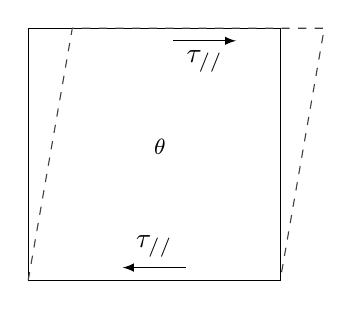
\begin{tikzpicture}[scale=0.8]
    \draw (-2,-2) rectangle (2,2);
    \draw[dashed,black!75!white] (-2,-2)--(-1.3,2)--(2.7,2)--(2,-2);

    \draw[-latex] (0.3,1.8)--(1.3,1.8);
    \node[below] at (0.8,1.8){$\tau_{//}$};
    \draw[-latex] (0.5,-1.8)--(-0.5,-1.8);
    \node[above] at (0,-1.8){$\tau_{//}$};

    \lPoint{A}{-1.3,2}
    \lPoint{B}{-2,-2}
    \lPoint{C}{-2,2}

    \lAngle[\text{\footnotesize $\theta$}]{A}{B}{C}[1][1.5]
\end{tikzpicture}
